\documentclass[12pt]{article}

%useful packages
\usepackage{color,soul}
\usepackage[usenames,dvipsnames,svgnames,table]{xcolor}
\usepackage{amsmath,amsthm,amscd,amssymb,bm}
\usepackage{hyperref}
\hypersetup{
    colorlinks=true,
    linkcolor=JungleGreen
}
\usepackage[utf8]{inputenc}
\usepackage[top=2cm, bottom=3cm, left=2cm, right=2cm]{geometry}
\usepackage{pgfplots}
\usepackage{enumitem}
\usepgfplotslibrary{fillbetween}
\usetikzlibrary{patterns}
\usepackage{tcolorbox}
\usepackage{centernot}
\usepackage{mathtools}
\usepackage{xcolor}

%personal definitions and commands
\newcommand{\R}{\mathbb{R}} 
\newcommand{\E}{\mathbb{E}}
\newcommand{\V}{\mathbb{V}}
\newcommand{\C}{\mathbb{C}}
\newcommand{\Prob}{\mathbb{P}}
\newcommand{\e}{\epsilon}
\newcommand\numberthis{\addtocounter{equation}{1}\tag{\theequation}} %allows numbering of single equations in align* environment
\newcommand{\mtx}[1]{\ensuremath{\bm{\mathit{#1}}}}
\newcommand{\B}{\hat{\boldsymbol{\beta}}}
\newcommand{\Cov}{\mathbb{C}\text{ov}}
\newcommand{\N}{\mathcal{N}}



\title{ECON611 -- Homework \# 2}
\author{Anirudh Yadav}
\setlength\parindent{0pt}
\begin{document}

\maketitle

%\setcounter{tocdepth}{2}
%\tableofcontents

\section{Maximum likelihood estimation of a simple DSGE model}

\subsection{} See attached code.

\subsection{}
\textbf{(a)} I plot the recovered structural shocks below.

\begin{figure}[h]
    \centering
        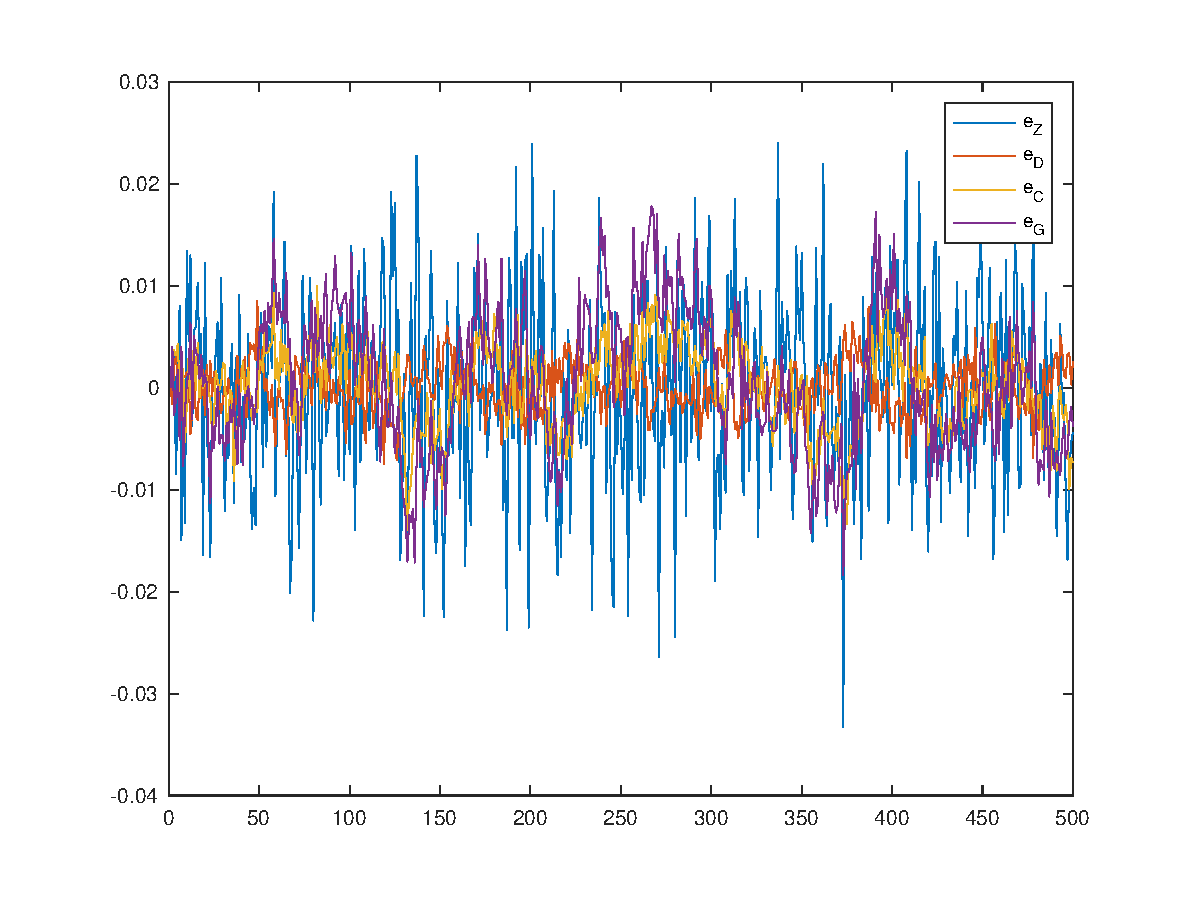
\includegraphics[width=0.6\textwidth]{shock_1.eps}
        \caption{Recovered Structural Shocks from the Brock-Mirman Model}
\end{figure}
To check the procedure I simulate shock processes for $\e_t = [\e_t^\delta, \e_t^c, \e_t^z, \e_t^g]$ and recover them. The recovered shocks are the same as the simulated shocks.\\

\textbf{(b)} I get $L =-6270.22$ (see attached code for details).\\

\textbf{(c) extra question.}
I plot the surface plot below.

\begin{figure}[h]
    \centering
        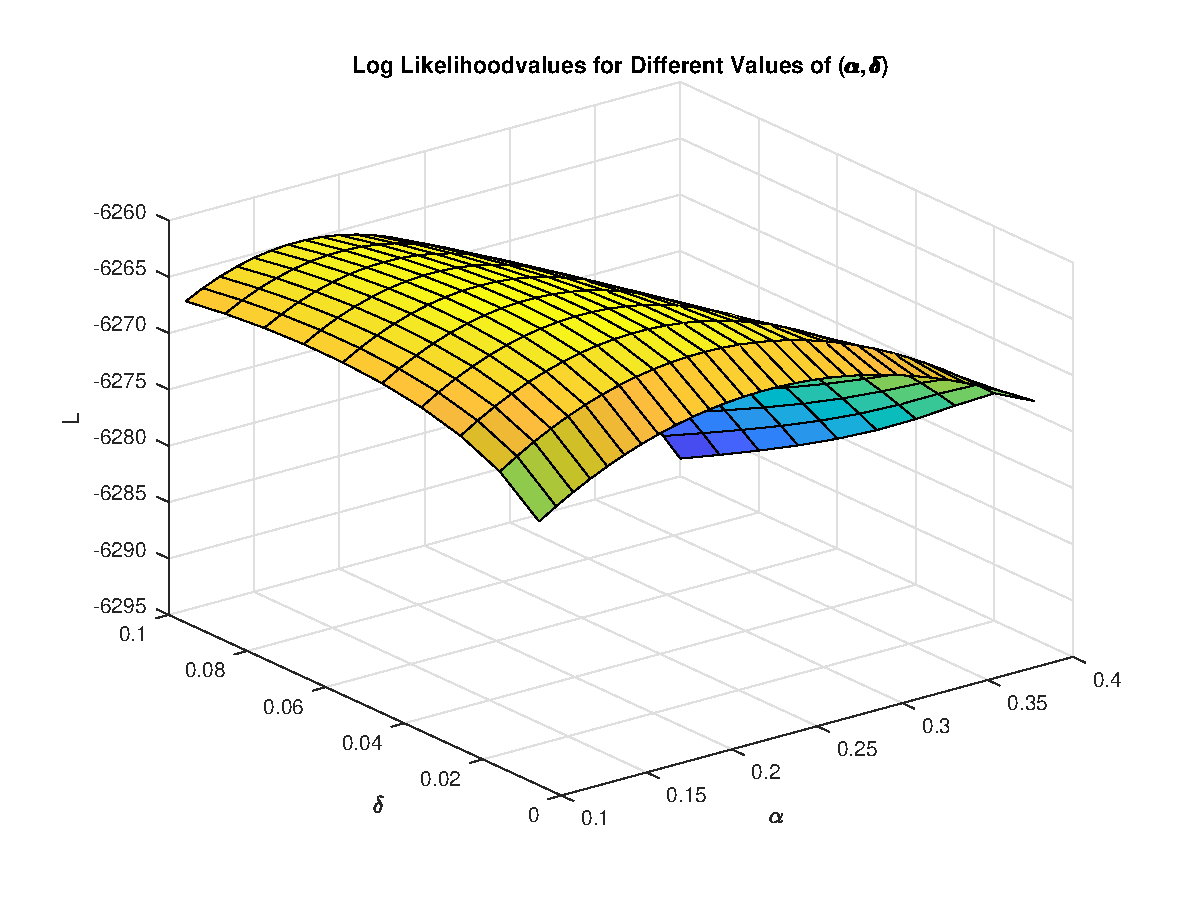
\includegraphics[width=0.8\textwidth]{surface.eps}
        \caption{Log-Likelihood Values for Different $(\alpha,\delta)$ Parameters}
\end{figure}

The likelihood is maximized at $(\alpha_{MLE},\delta_{MLE}) = (0.2,0.05)$, which doesn't correspond to our usual calibration. Interestingly, the likelihood seems quite flat, which we talked about in class.


\newpage

\section{An endowment economy}

\subsection{}
Both types of agents face identical problems. They solve
\begin{align*}
&\max_{c, s} \sum_{t=0}^\infty \beta^t \ln(c_t)\\
&\text{s.t } c_t + s_t = y_t + (1+r_{t-1})s_{t-1}\\
&\text{\& } s^A_t + s^B_t = 0.
\end{align*}

Since there is no uncertainty, the Bellman is 
\begin{align*}
V(s_{-1} , y) = \max_s \{ \ln(y+(1+r_{-1})s_{-1} - s) + \beta V(s,y')\}.
\end{align*}
Combining the FOC wrt $s$, with the B-S condition gives the following optimality condition
\begin{align}
\frac{1}{c_t} = (1+r_t)\beta \frac{1}{c_{t+1}} \text{ } \label{eq:1}
\end{align}
Now, a competitive equilibrium is a sequence of allocations $\{c^i_t, s^i_t\}_{t,i}$ such that each agent's optimality condition (\ref{eq:1}) and budget constraint hold each period, given a sequence of interest rates $\{1+r_t\}_t$, and the bond market clears each period. It is easy to guess and verify that an equilibrium exists where for each agent, $c_t = 1$, $s_t = 0$ and $(1+r_t) = 1/\beta$ for all $t$. Clearly, this allocation satisfies the optimality condition and the budget constraint (since $c_t = y_t$ each period) and bond market clearing (since neither agent saves/borrows). Thus, in the competitive equilibrium, both agents consume their endowments each period, and there are no gains from trade.

\subsection{}
Neither agent will react to this news in period 0. The only plausible reaction to the news would be for agents to borrow against potentially higher income next period (there is no way that this news could induce a savings response). But both agents want to make the same trade, since they are identical before the shock. Obviously, both agents cannot increase their borrowing simultaneously in period zero because this would contradict bond market clearing. Thus, in equilibrium, neither agent reacts to the news in period zero.

\subsection{}
This problem is essentially the same as the 2 country IRBC example we looked at in class.\\ 

I'm not sure exactly how to solve for the time paths by hand, but here's the intuition. Consider agent $A$, who gets the positive income shock. She wants to amortize this shock over her lifetime like a good PIH agent would do. To do so, she needs to save in period 1, which must mean that agent $B$ has to borrow in equilibrium. Thus, consumption of both agents increase in period 1. Next, note that if agent $B$ does nothing (i.e. just consumes her endowment every period), her lifetime utility is zero. Thus, agent $A$ chooses her savings in period 1 such that taking the other side of the bond trade gives $B$ a lifetime utility of exactly zero (I think this explains why $A$'s consumption isn't perfectly smooth). Thus, we get the pattern we saw in class: both agents have higher consumption in period 1; for $t\geq 2$, $A$'s consumption remains above 1 forever, and $B$'s is slightly below 1 forever. 

\iffalse
The present value of agent $A$'s endowment at $t=1$ is
\begin{align*}
\sum_{j=0}^\infty \beta^jy^A_{t+j} &= 2 + \beta(1) + \beta^2(1) + \beta^3(1)+...\\
&= 1 + \frac{1}{1-\beta}
\end{align*}
The annuity value $\bar c^A$ that has the same value as this endowment stream is 
\begin{align*}
\frac{\bar c^A}{1-\beta} &= 1 + \frac{1}{1-\beta}\\
\implies \bar c^A &=1 + (1-\beta) = 2-\beta.
\end{align*}
I shall guess and verify that in equilibrium $c_t^A =\bar c^A$ for all $t$. First note that the associated savings scheme comes from the budget constraint. Under the proposed allocation, $A$'s period 2 budget constraint is
\begin{align*}
c_2^A + s^A_2 = y^A_2 + (1+r_1)s^A_1
\end{align*}
And since $c_1^A = c_2^A =\bar c^A  =2-\beta$ we must have $s_1 = \beta$. Thus, 
\begin{align*}
\bar c^A + s^A_2  &=1 + 1 \text{ with } 1+r_1 = 1/\beta\\
\implies s^A_2 &= \beta.
\end{align*}
Following this logic, it is pretty easy to see that $s_t^A = \beta$ for all $t \geq 1$. Bond market clearing then implies that $s_t^B = -\beta$ for all $t$. So we have the following allocations
\begin{align*}
c_t^A &= 2-\beta, s_t^A = \beta\\
c_t^B &= 1+\beta, s_t^B = -\beta
\end{align*}
for all $t$, with $(1+r_t) = 1/\beta$ for all $t$. Clearly, these allocations satisfy the agents' optimality condition (\ref{eq:1}) (since no agent is borrowing constrained), budget constraints, and bond market clearing; so it is an equilibrium.
\fi


\subsection{}
The equilibrium conditions of the model are
\begin{align}
\frac{1}{c^i_t} &=(1+r_t)\beta \frac{1}{c^i_{t+1}}\\
c^i_t + s^i_t &= y^i_t + (1+r_{t-1})s^i_{t-1}\\
y_t^i &= 1 + e^i_t \\
s^A_t + s^B_t &=0
\end{align}
for $i \in \{A,B\}$.\\

The non-stochastic steady state is given by
\begin{align*}
\bar c_A &= \bar c_B = \bar y_A = \bar y_B =1\\
\bar s_A &= \bar s_B = 0\\
1+\bar r &= 1/\beta
\end{align*}
Log-linearizing around the steady state gives the following system of 7 equations with 7 variables:
\begin{align}
-\tilde c_t^i &= \beta \tilde r_t - \tilde c^i_{t+1} (\text{where } \tilde r_t = r_t - \bar r) &\textcolor{blue}{\text{ (`euler')}} \\
\tilde c_t^i + s_t &= \tilde y^i_t + (1+\bar r) s^i_{t-1} &\textcolor{blue}{\text{ (`budget constraint')}}\\
\tilde y^i_t &= e^i_t  &\textcolor{blue}{\text{ (`income process')}}\\
s^A_t + s^B_t &=0 &\textcolor{blue}{\text{ (`bond mkt clearing')}}
\end{align}
We consider a one-time shock to $A$'s income in period 1. I plot the time paths for $\tilde c^A_t,\tilde c^B_t, s^A_t, s^B_t$ and $r_t$ overleaf.

\begin{figure}[h]
    \centering
    \begin{minipage}{0.5\textwidth}
        %\centering
        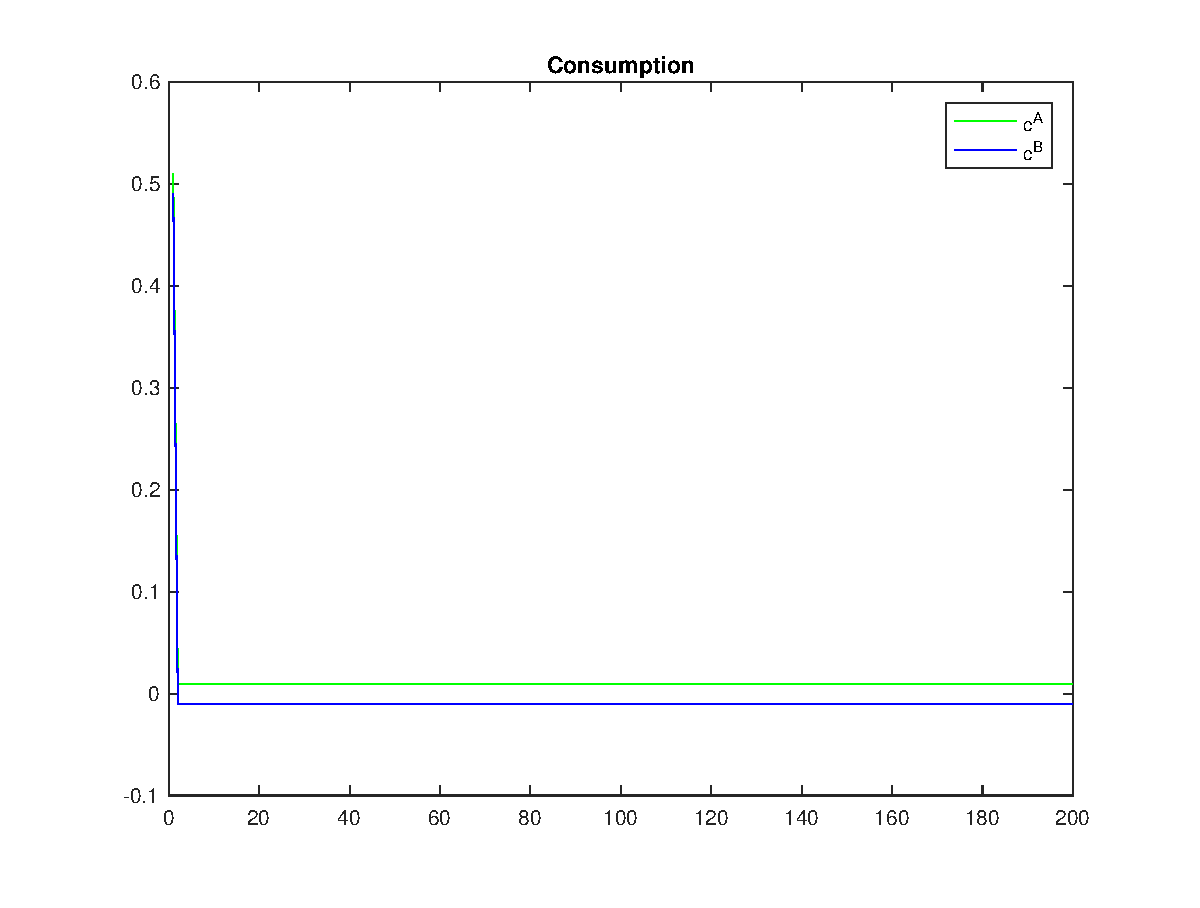
\includegraphics[width=1\textwidth]{IRF_c.eps}
        \caption{Consumption}
    \end{minipage}\hfill
    \begin{minipage}{0.5\textwidth}
      %  \centering
        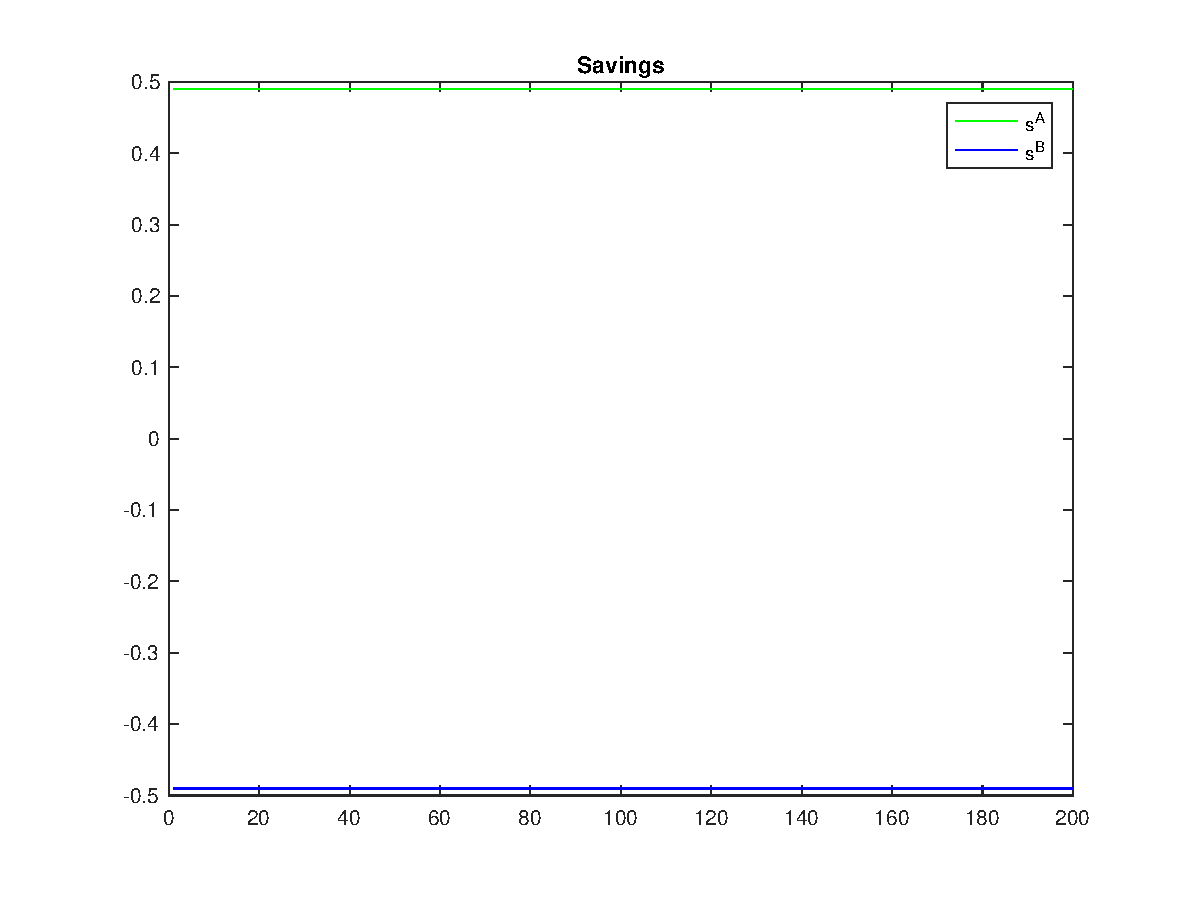
\includegraphics[width=1\textwidth]{IRF_s.eps}
        \caption{Savings}
    \end{minipage}
\end{figure}

\begin{figure}[h]
    \centering
        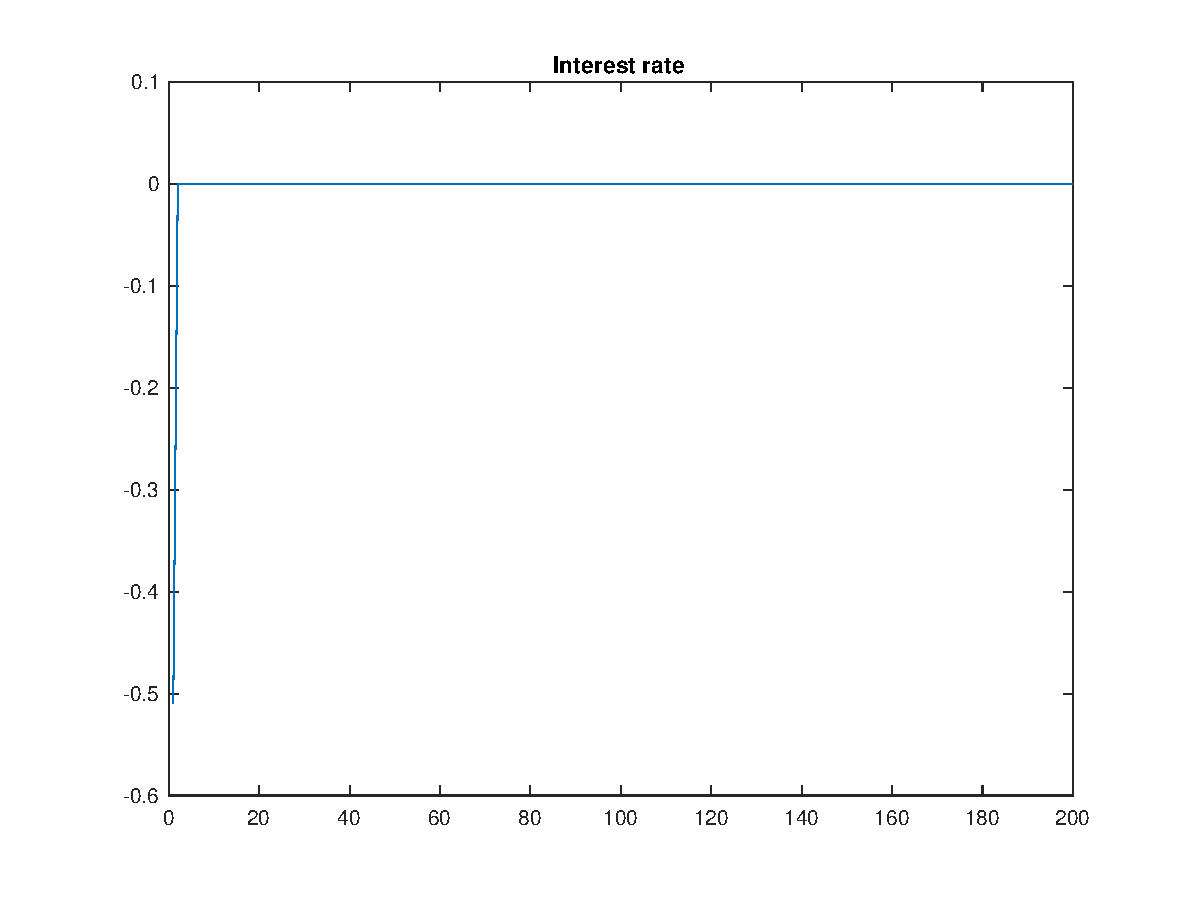
\includegraphics[width=0.5\textwidth]{IRF_r.eps}
        \caption{$r_t$}
\end{figure}
 
\subsection{} I'm guessing that $(1+r_0)$ increases at the time of the announcement in period 0 because both agents want to borrow.

\newpage

\section{The Kalman Filter}
\subsection{}
The Kalman Filter works as follows
\begin{enumerate}
\item \textit{Initialization:} with $\rho=0.8$ our initial assesment is $\hat y_{1|0} = 0$ and $V_{1|0} = \frac{\sigma^2_e}{1-\rho^2}$. 
\item \textit{Forecast of $x_t$:} the optimal date $t$ forecast of the observable is $\hat x_{t|t-1} = \hat y_{t|t-1}$. Pick up the associated MSE
\begin{align*}
\E[(x_t - \hat x_{t|t-1})^2] = V_{t|t-1} + \sigma^2_m.
\end{align*}
\item \textit{Update forecast of $y_t$:} the updated forecast of $y_t$ given observed data $x_t$ is
\begin{align*}
\hat y_{t|t} = \hat y_{t|t-1} + V_{t|t-1}[V_{t|t-1} + \sigma^2_m]^{-1}(x_t - \hat y_{t|t-1})
\end{align*}
\item \textit{Compute forecast of $y_{t+1}$ given $x_t$}:
\begin{align*}
\hat y_{t+1|t} = \rho \hat y_{t|t} = \rho \hat y_{t|t-1} + \rho V_{t|t-1}[V_{t|t-1} + \sigma^2_m]^{-1}(x_t - \hat y_{t|t-1})
\end{align*}
\item \textit{Iterate.}
\end{enumerate}

\end{document}
